\section{Datos y Métodos}

\begin{frame}{El tamaño del CT}
\textbf{¿Qué es el tamaño de los CTs?} \\ El término tamaño del CT suele ser muy ambiguo porque se puede abordar diferentes parametrizaciones considerando principalmente:
\begin{itemize}
    \item La velocidad del viento de los CTs
    \begin{itemize}
        \item Intensidad de los vientos en su circulación interna
        \item Intensidad de los vientos en su circulación externa
    \end{itemize}
    \item La vorticidad
    \item Isobaras (curva de igual o constante presión)
    \item Precipitación reportada a ciertos umbrales
\end{itemize}

\end{frame}

\subsection{Bases de datos utilizadas}
\begin{frame}
    \begin{block}{Para calcular el tamaño}
        \begin{itemize}
            \item Posiciones del CT cada 6 h HURDAT
            \item Productos IR del GPM
            \item Tamaño del campo de vientos.
        \end{itemize}
    \end{block}

    \begin{exampleblock}{Para validar relación entre el tamaño y precipitación}
        \begin{itemize}
            \item Producto satelital GPM\_IMERG
            \item Producto de precipitación CHIRPS
        \end{itemize}
    \end{exampleblock}

    \begin{alertblock}{Para la validación de las variables ambientales con la precipitación}
    Se utilizaron las siguientes variables: 
    Velocidad vertical del viento a 500 hPa, humedad específica a 600 hPa, vorticidad a 200 hPa, divergencia a 200 hPa, cizalladura del viento, contenido total de agua precipitable
    \end{alertblock}
\end{frame}

\subsection{ROCLOUD: Una nueva aproximación del tamaño del CT}
\begin{frame}
    \begin{block}{Sobre el tamaño de la circulación del CT}
        Pérez-Alarcón et al. (2021) desarrollaron una base de datos sobre el tamaño de los CTs utilizando los perfiles uniformes del viento descritos por Willoughby et al. (2006). \bigskip

        Estos cálculos utilizan la posición del CT obtenida del HURDAT2, la intensidad máxima de los vientos y el radio de los vientos máximos, calculado a través de modelos específicos para cada cuenca o en función de la posición latitudinal del CT.

    \begin{equation}
        \label{eq:2.1}
        r_{m} =  46.6 \ \exp{(-0.015 \ V_{max} + 0.0169 \phi)}
    \end{equation}
        \\~\
    \end{block}

\end{frame}

\begin{frame}
    Se diseñó un algoritmo que mide las distancias radiales desde el centro del CT hasta el punto más alejado donde las temperaturas de brillo de las nubes pertenecen a la circulación del CT y están por debajo de -40°C
    \\~\ 
    \\~\ 
\begin{enumerate}
    \item<1-> Segmentación a -40°C
     \\~\
    \item<2-> Selección de regiones de intéres
     \\~\
    \item<3-> Selección de poligonos dentro del campo de vientos
     \\~\
    \item<4-> Determinación de los radios por cuadrante
     \\~\
    \item<4-> Cálculo del radio promedio
\end{enumerate}
\end{frame}

\begin{frame}
    \begin{figure}
        \centering
        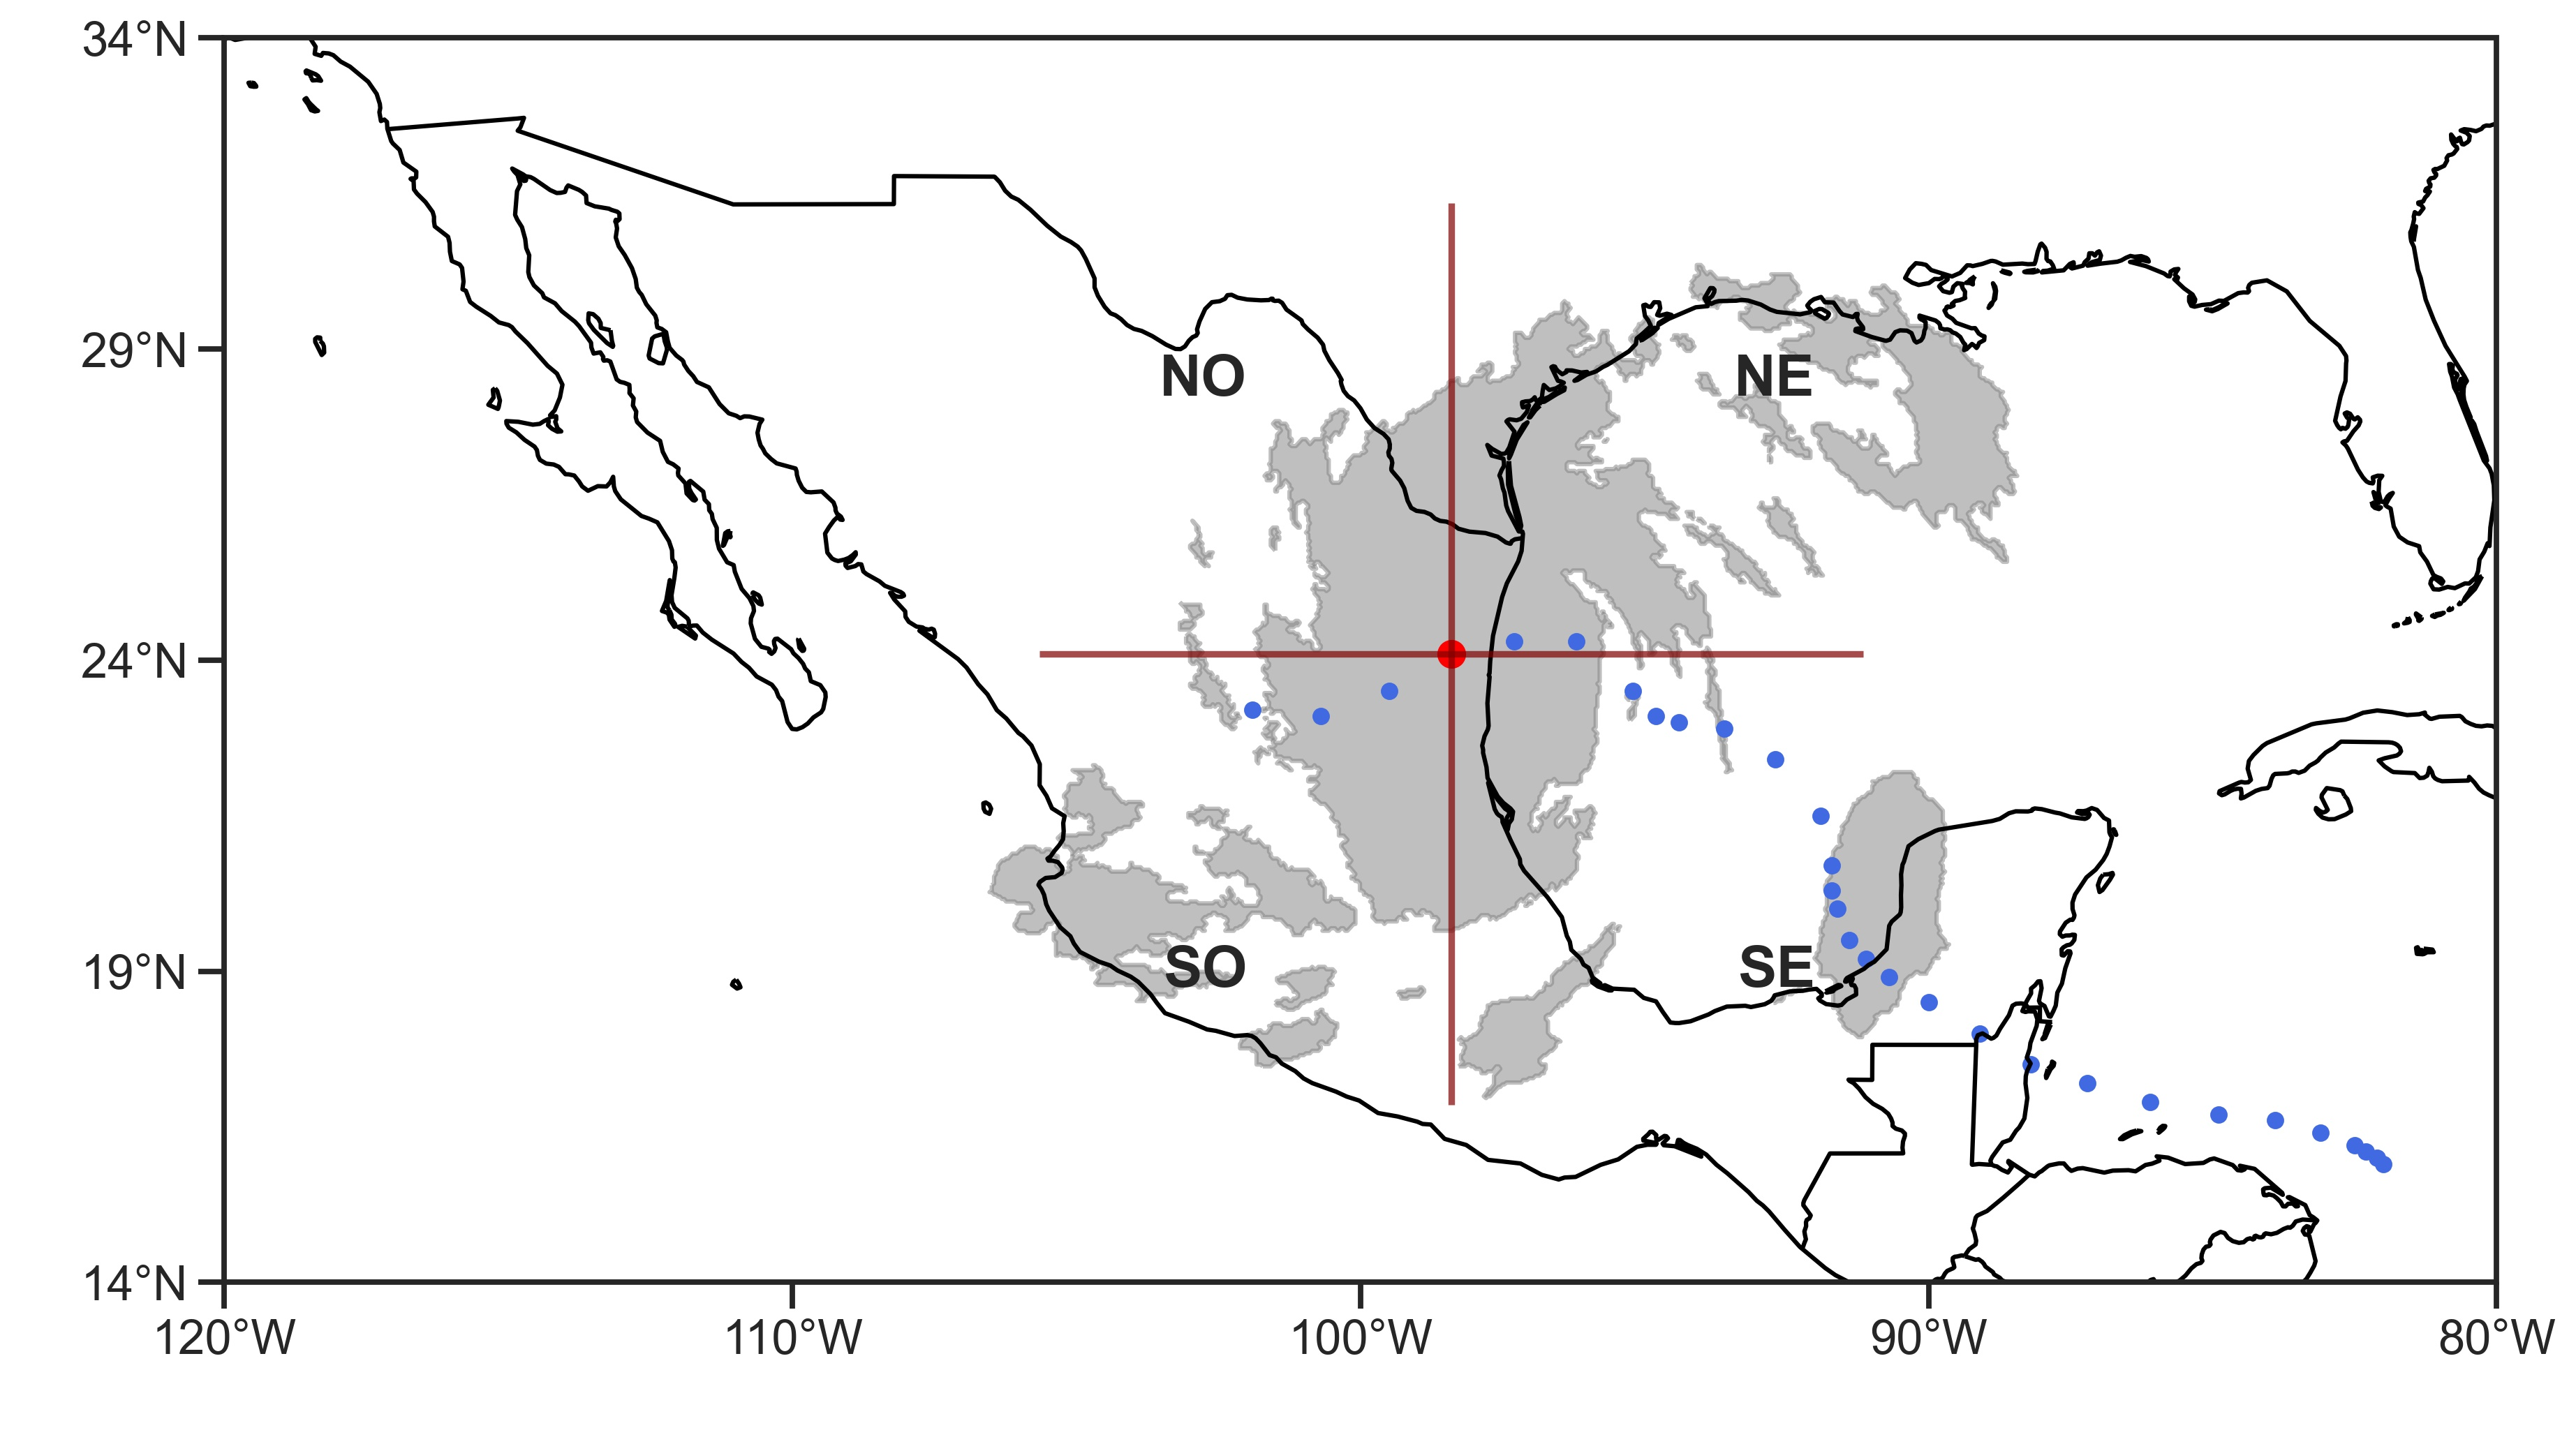
\includegraphics[scale = 0.32]{Images/Figures/Fig_2_3.jpeg}
        \caption{Extensión del campo de nubes a través de contornos generados con imágenes IR (contornos grises) del huracán Alex 2010, cuyas posiciones están representadas por puntos azules}
        \label{fig:fig_5}
    \end{figure}
\end{frame}

\subsection{Métodos para relacionar la lluvia con el tamaño del ciclón}
\begin{frame}
\begin{enumerate}
\setcounter{enumi}{0}
\item Algoritmo del Radio de las Bandas de Precipitación
(RBP)
      \begin{figure}
            \centering
            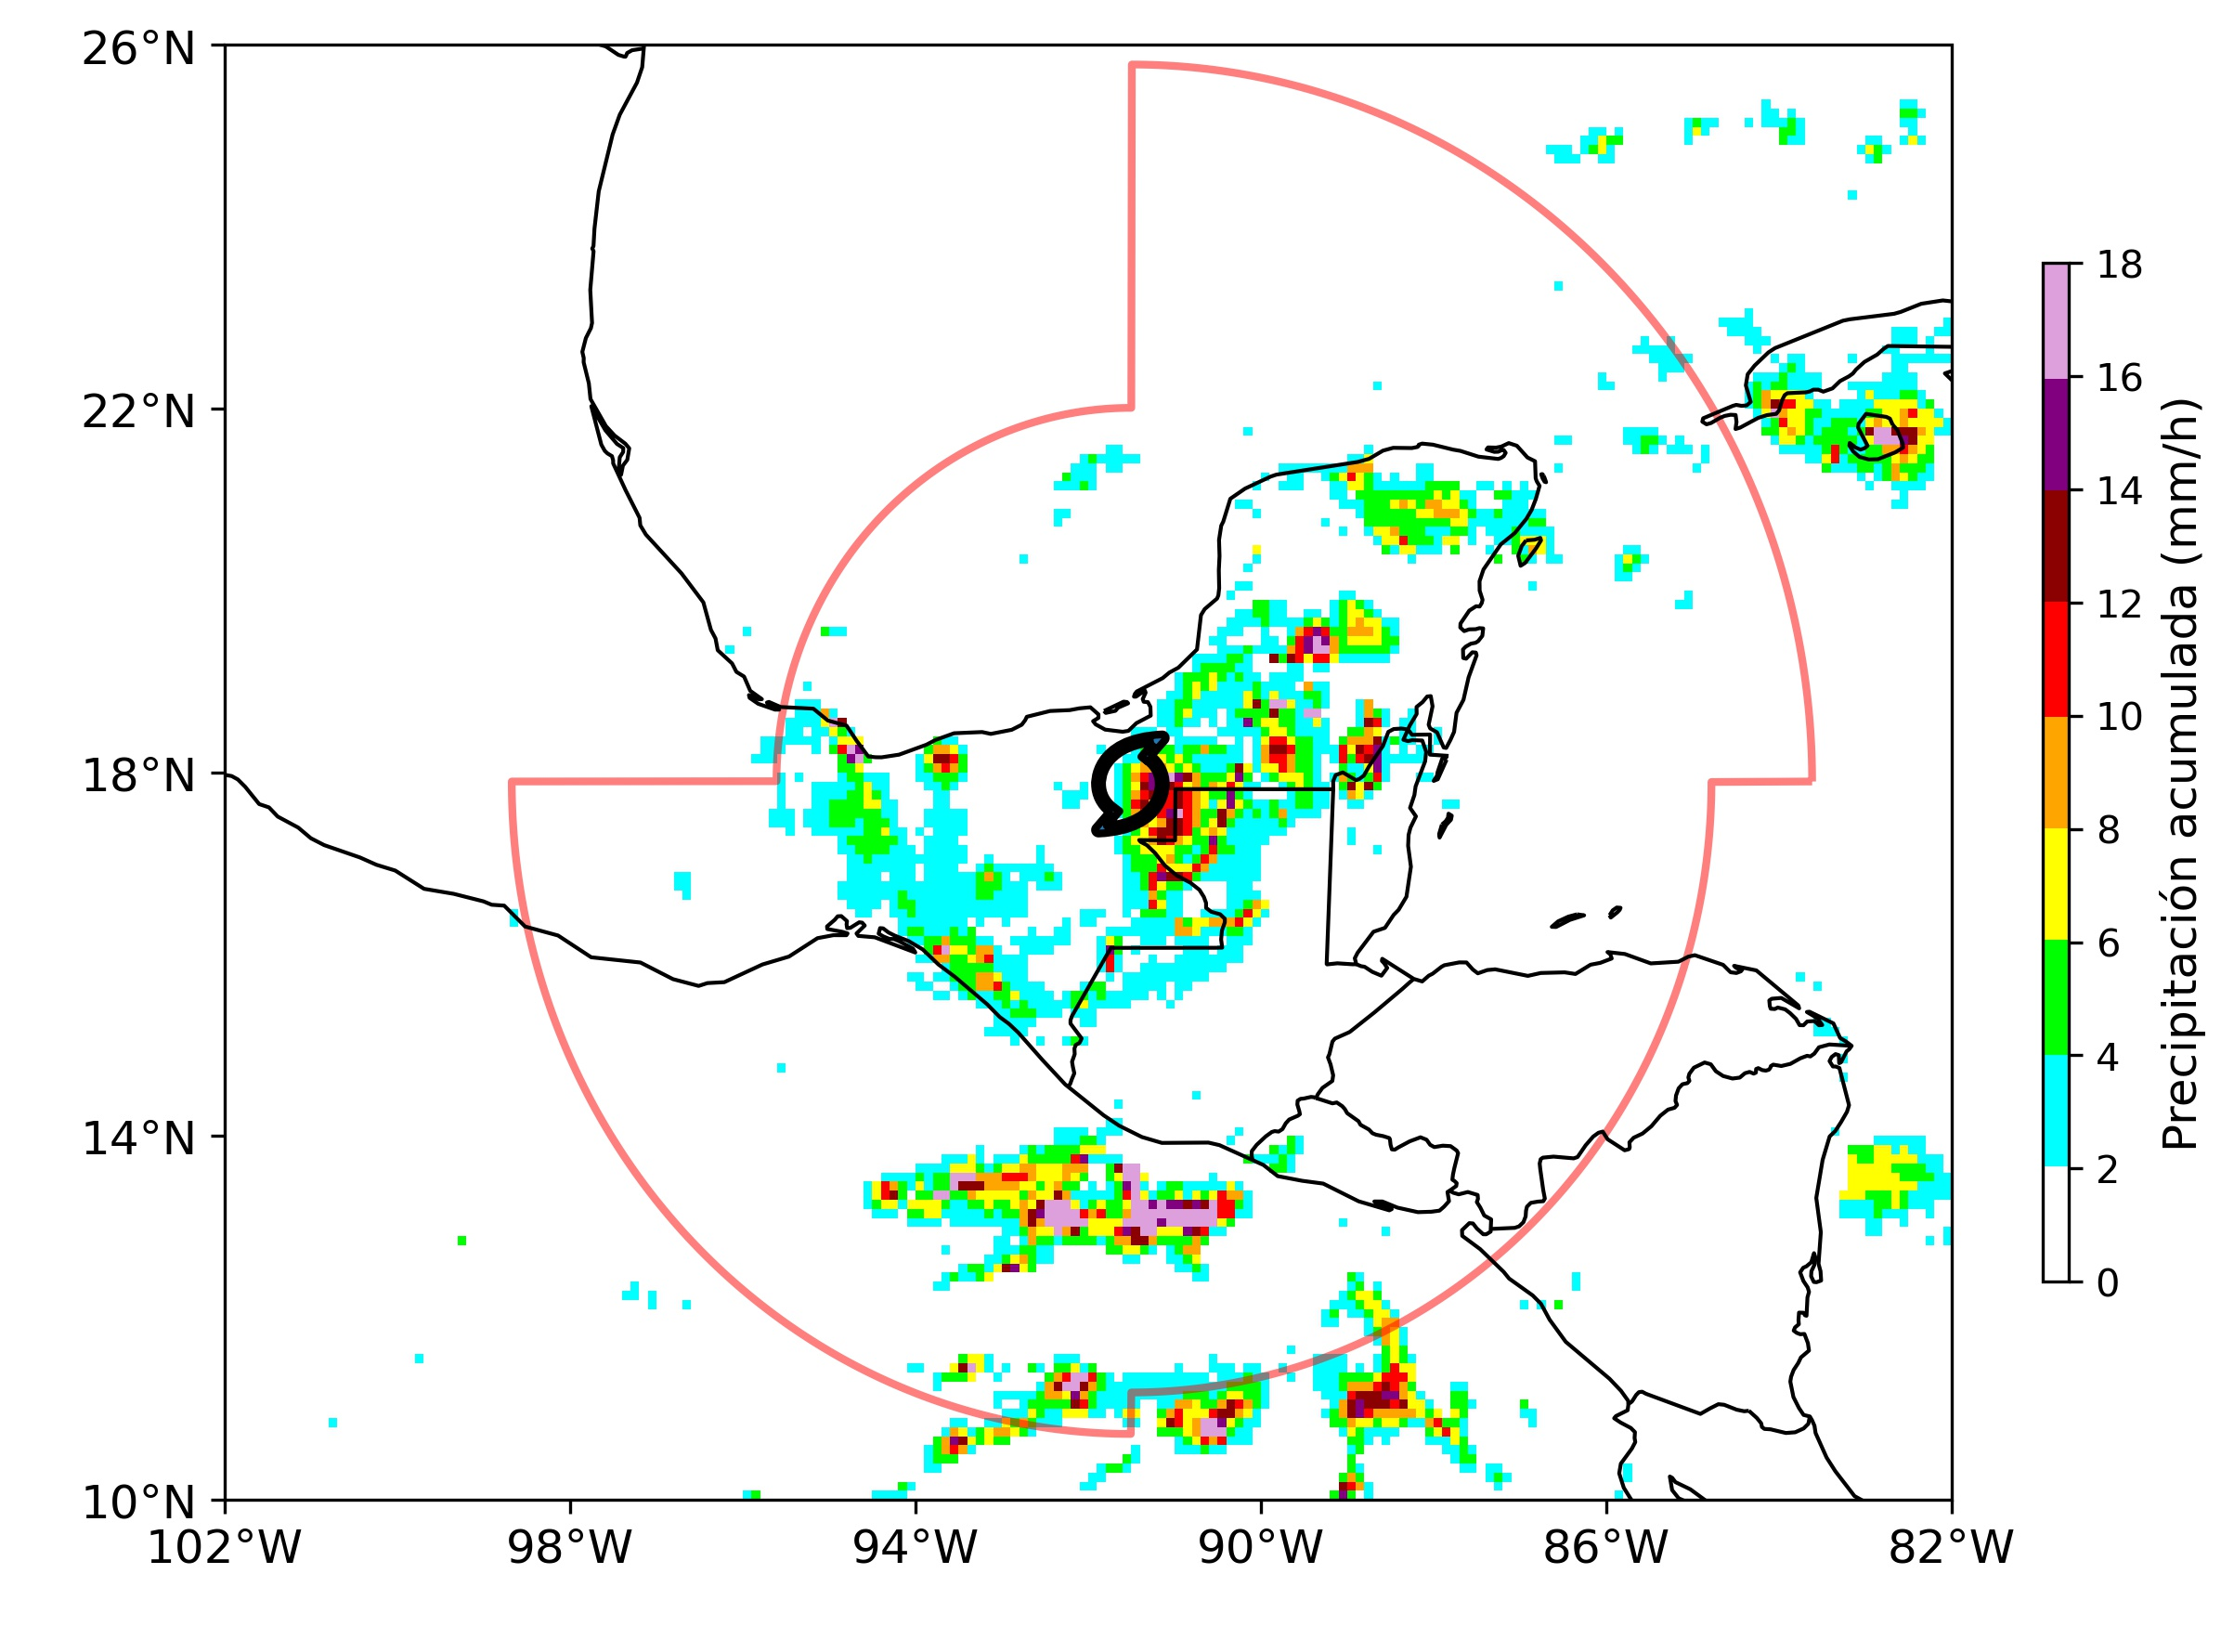
\includegraphics[scale = 0.39]{Images/Figures/Fig_2_5.jpeg}
            \caption{Valores de precipitación del GPM\_IMERG para la TT Cristóbal en su posición del 4 de junio del 2020 a las 06:00 UTC.}
            \label{fig:fig_6}
        \end{figure}
\end{enumerate}
\end{frame}

\begin{frame}
\begin{enumerate}
\setcounter{enumi}{1}
\item Técnica de anillos usando los datos de GPM\_IMERG
      \begin{figure}
            \centering
            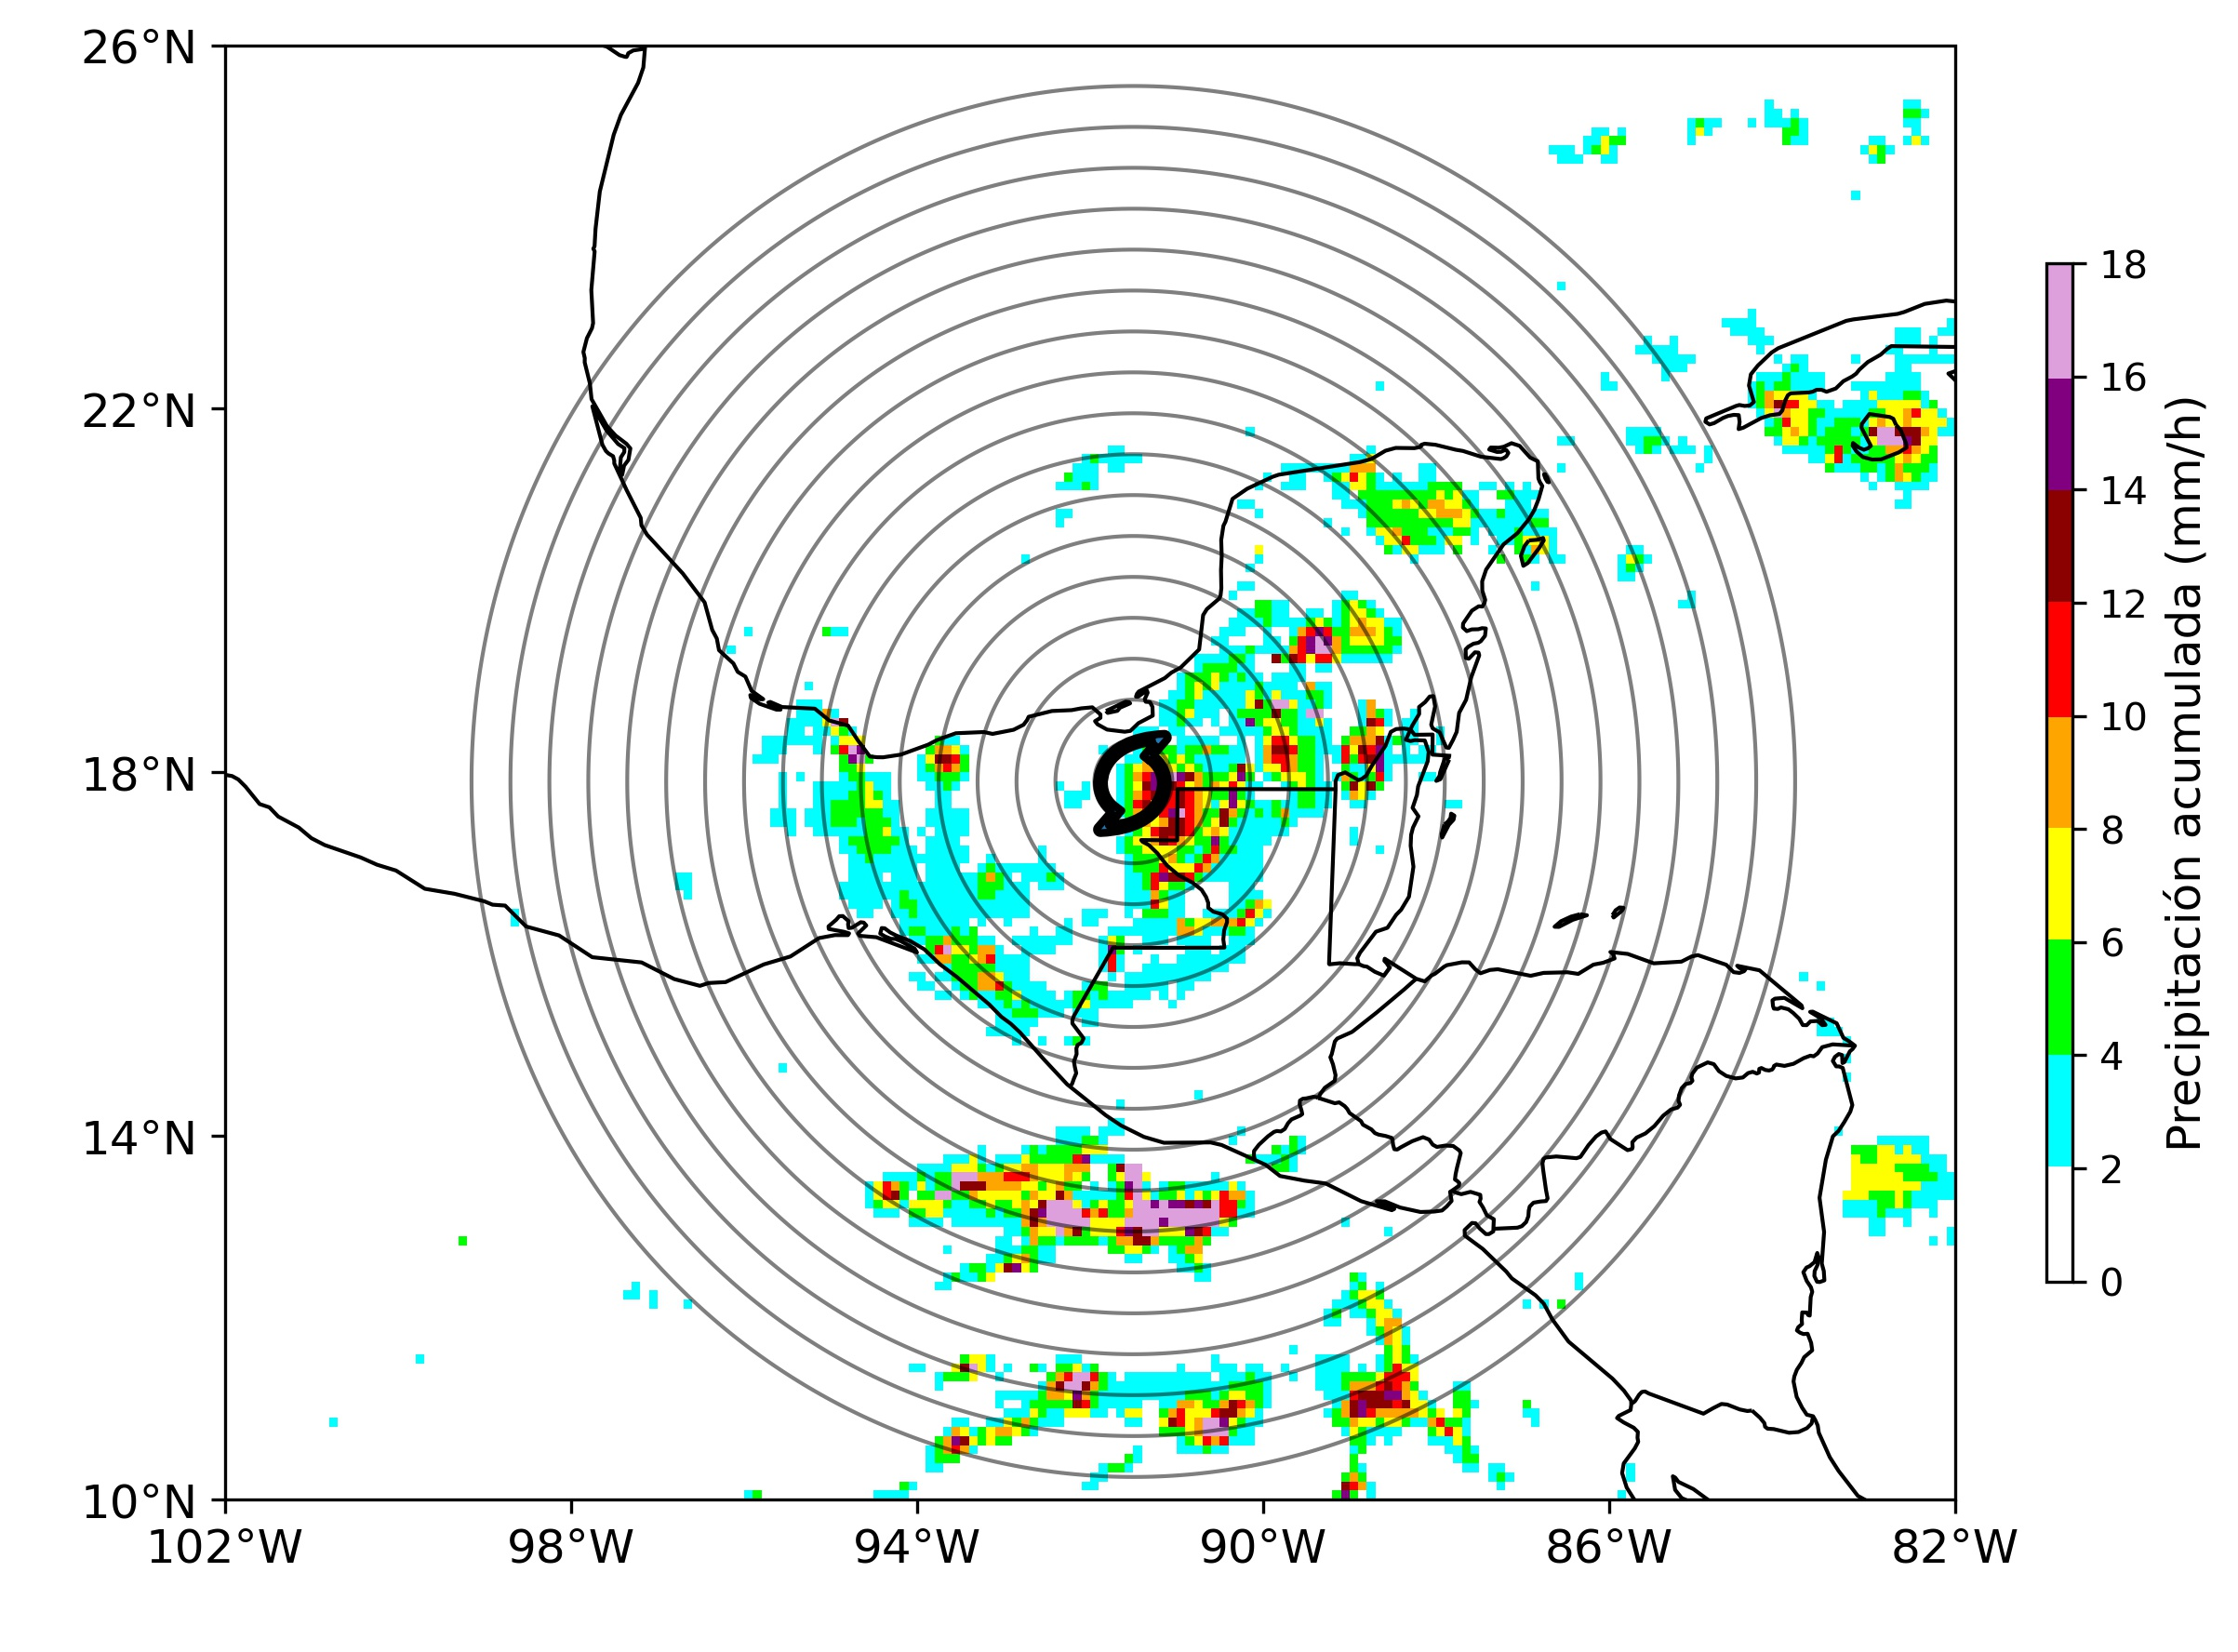
\includegraphics[scale = 0.4]{Images/Figures/Fig_2_6.jpeg}
            \caption{Similar a la Fig. \ref{fig:fig_6}, pero mostrando los anillos usados cada 50 km.}
            \label{fig:fig_7}
        \end{figure}
\end{enumerate}
\end{frame}

\begin{frame}
\begin{enumerate}
\setcounter{enumi}{2}
\item Técnica de anillos usando los datos continentales de CHIRPS
      \begin{figure}
            \centering
            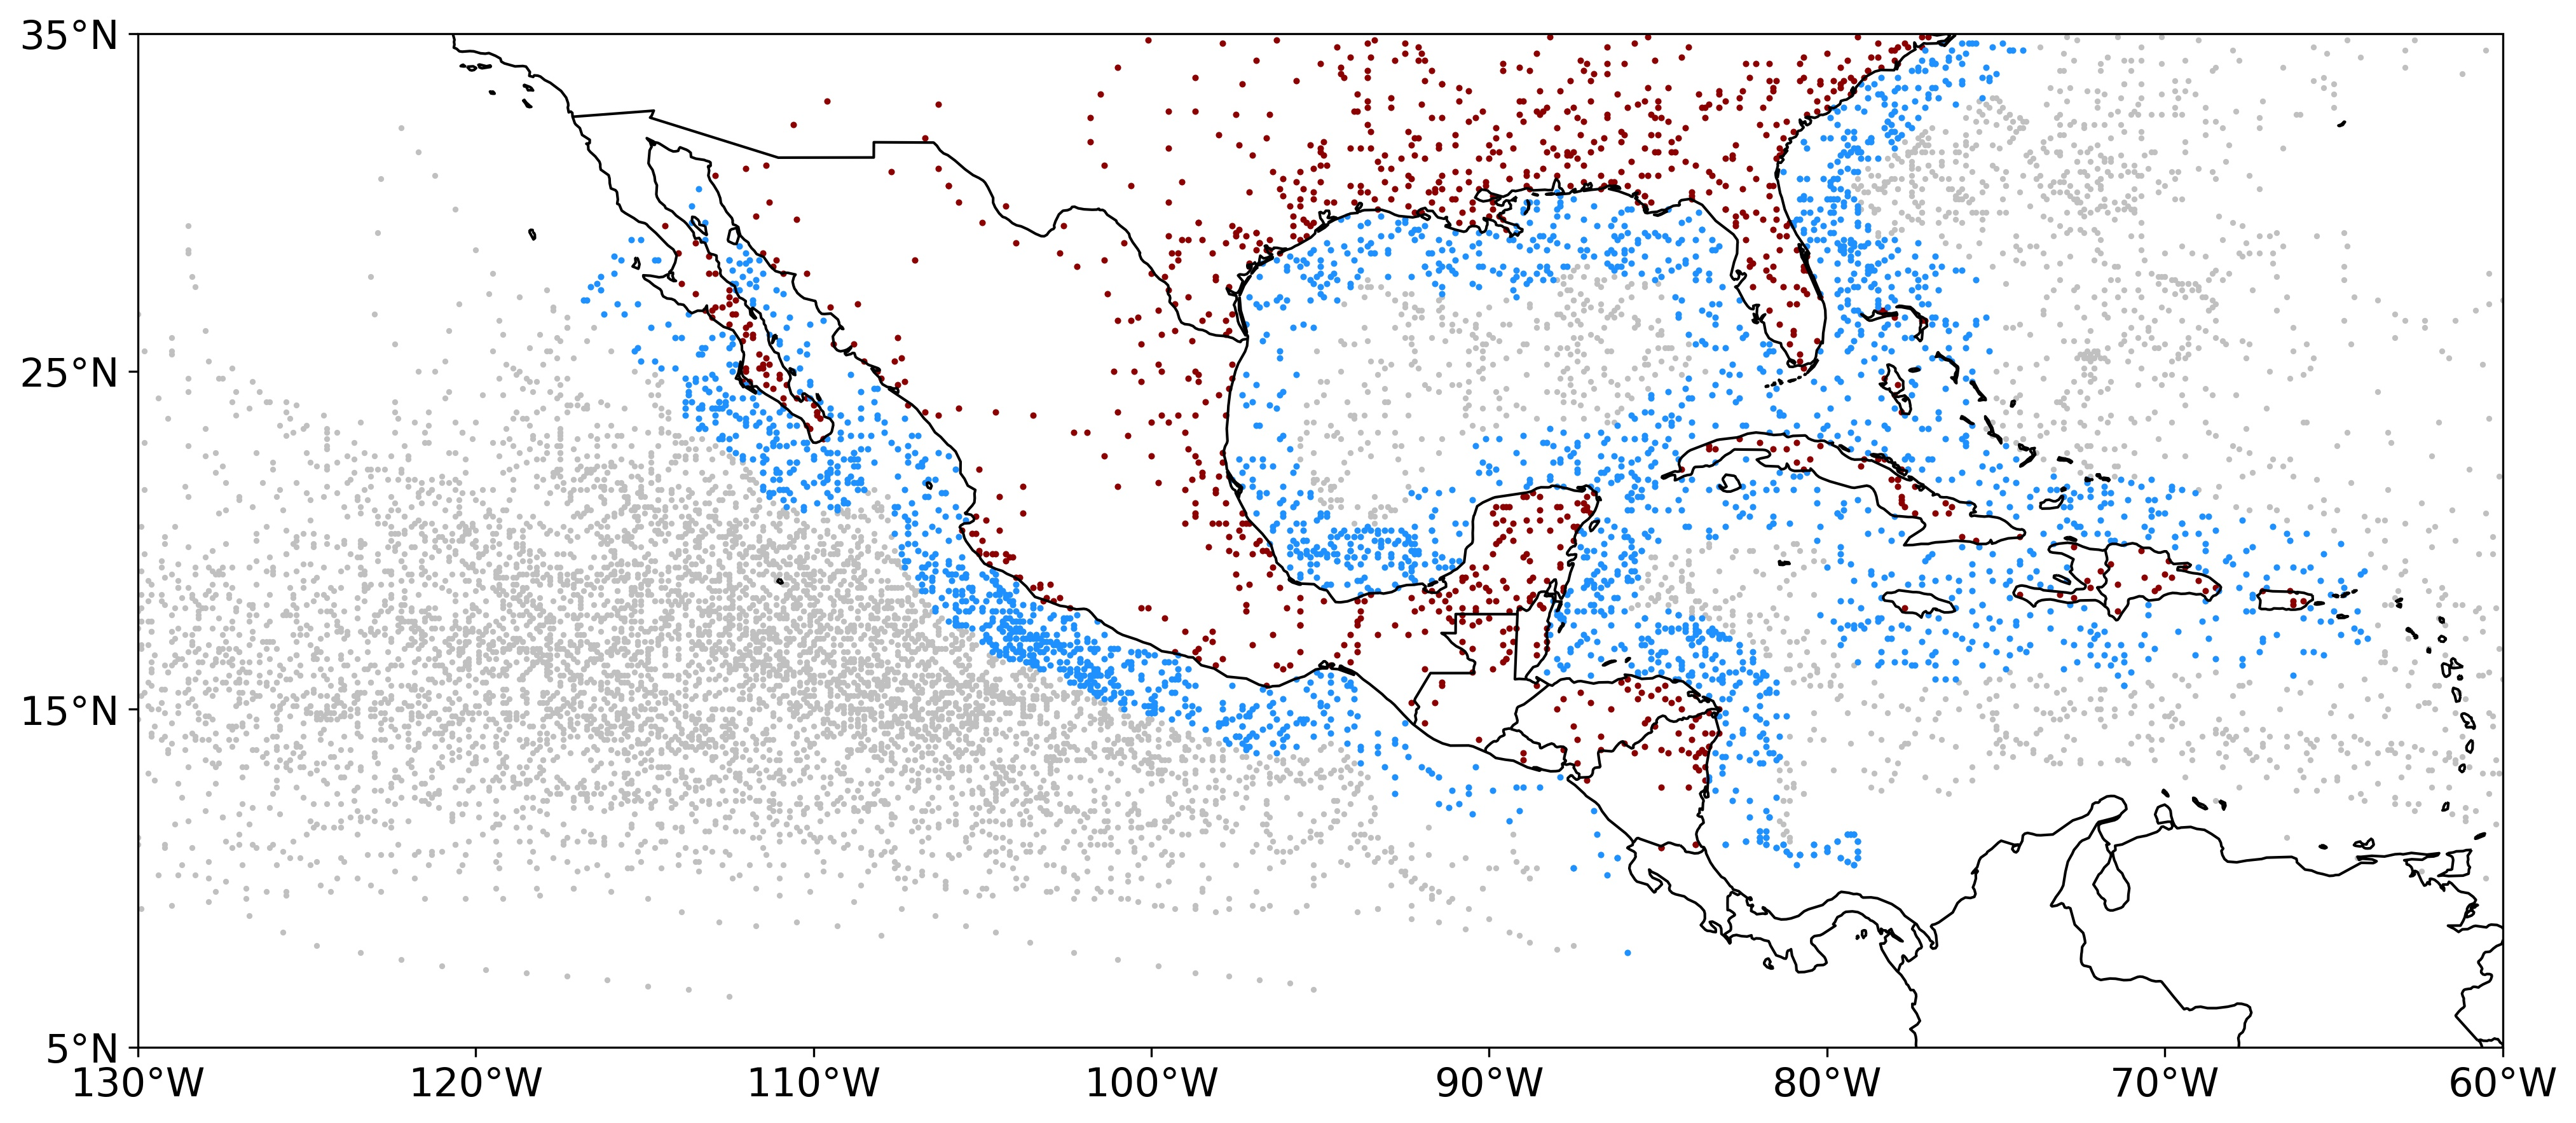
\includegraphics[scale = 0.24]{Images/Figures/Fig_2_7.jpeg}
            \caption{Posiciones de los CT que se encuentran sobre territorio mexicano (rojo) y cercanos a la costa (distancia a 250 km, en azul).}
            \label{fig:fig_8}
        \end{figure}
\end{enumerate}
\end{frame}

\subsection{Sobre las variables medioambientales y la forma}

\begin{frame}
    \begin{alertblock}{Relaciones estadísticas}
        \begin{enumerate}
            \item Correlación Spearman
            \item Modelos de Estimación de Ecuaciones Generalizadas
        \end{enumerate}
        ~\
    \end{alertblock}
~\
    
    \begin{exampleblock}{La forma del CT}
        \begin{enumerate}
            \item Dispersión
            \item Asimetría
            \item Solídez
        \end{enumerate} 
        ~\
    \end{exampleblock}
\end{frame}
